% TODO
%\begin{itemize}
%	\item $>= 1$ Entwurfsmuster einsetzen und begründen
%	\item UML-Diagramm vorher und nachher
%\end{itemize}

Entwurfsmuster befassen sich mit der Lösungsansätzen für wiederkehrende Entwurfsprobleme.
Sie sind somit eine Standardvorlage um Probleme zu umgehen.
Dies geschieht auf einer höheren Abstraktion als objekt-orientierte Programmierung selbst.\\
Grundlegend lassen diese Entwurfsmuster in vier Kategorien einordnen: Erzeugungsmuster (Erstellung von Instanzen), Strukturmuster (Vereinfachung des Designs), Verhaltensmuster (Zusammenarbeit von Komponenten) und Nebenläufigkeitsmuster (Multithreading).

Im folgenden wird die Anwendung eines Verhaltensmusters in unserem Programm erklärt.

\paragraph{Beobachter}
Das im Code identifizierte Entwurfsmuster ist das objektbasierte Verhaltensmuster \enquote{Beobachter}.
Hierbei registriert sich in der \texttt{Start()} Methode der Klasse \texttt{UpdateTimer} dieser auf das \texttt{Elapsed} Event des \texttt{Timers}.
Hierbei wird die Methode \texttt{RefreshCallback()} angemeldet.
Diese delegiert den Methodenaufruf an die Klasse \texttt{Refresher}, um das Hintergrundbild zu ändern.
Der \texttt{Timer} ist das Subjekt, bei welchem sich der \texttt{UpdateTimer} anmeldet.

Das folgende UML Diagramm zeigt beide Klassen und ihren Zusammenhang:

\medspace
\begin{figure}[h]
	\begin{center}
		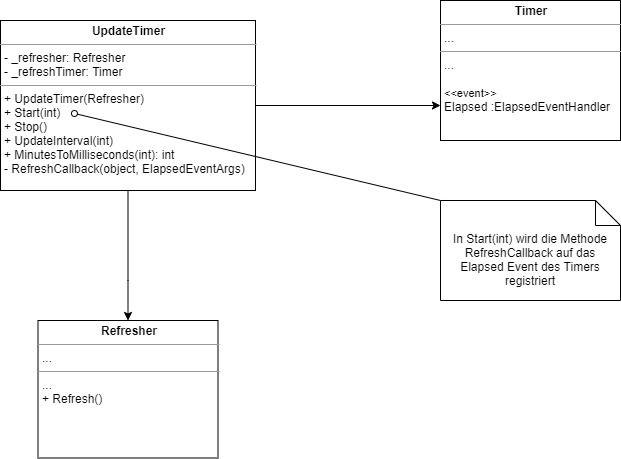
\includegraphics[width=\linewidth]{Bilder/Beobachter_UML.png}
	\end{center}
	\caption{UML Diagramm des Entwurfsmuster \enquote{Beobachter}}
\end{figure}